\section{Complementary Material Controller Design}
\begin{figure}[tbh]
	\centering
	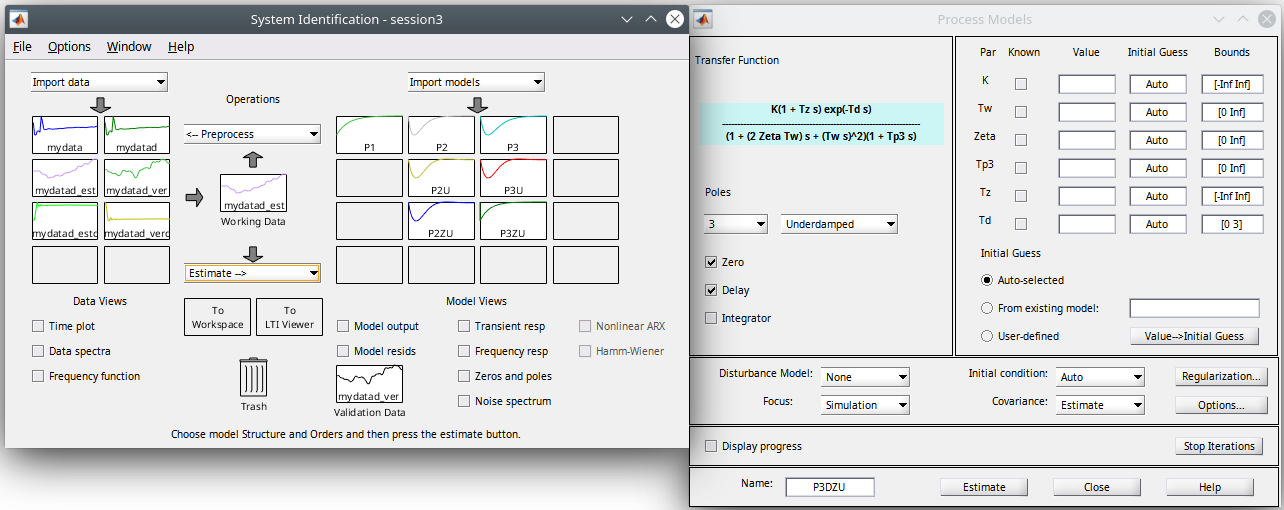
\includegraphics[width=\textwidth]{chap/Appendix/ControllerDesign/identi}
	\caption[Matlab System Identification Toolbox]{Screenshot of the Matlab System Identification Toolbox; to the right the process models estimator window}
	\label{fig:Appendix-identify}
\end{figure}

\begin{figure}[tbh]
	\centering
	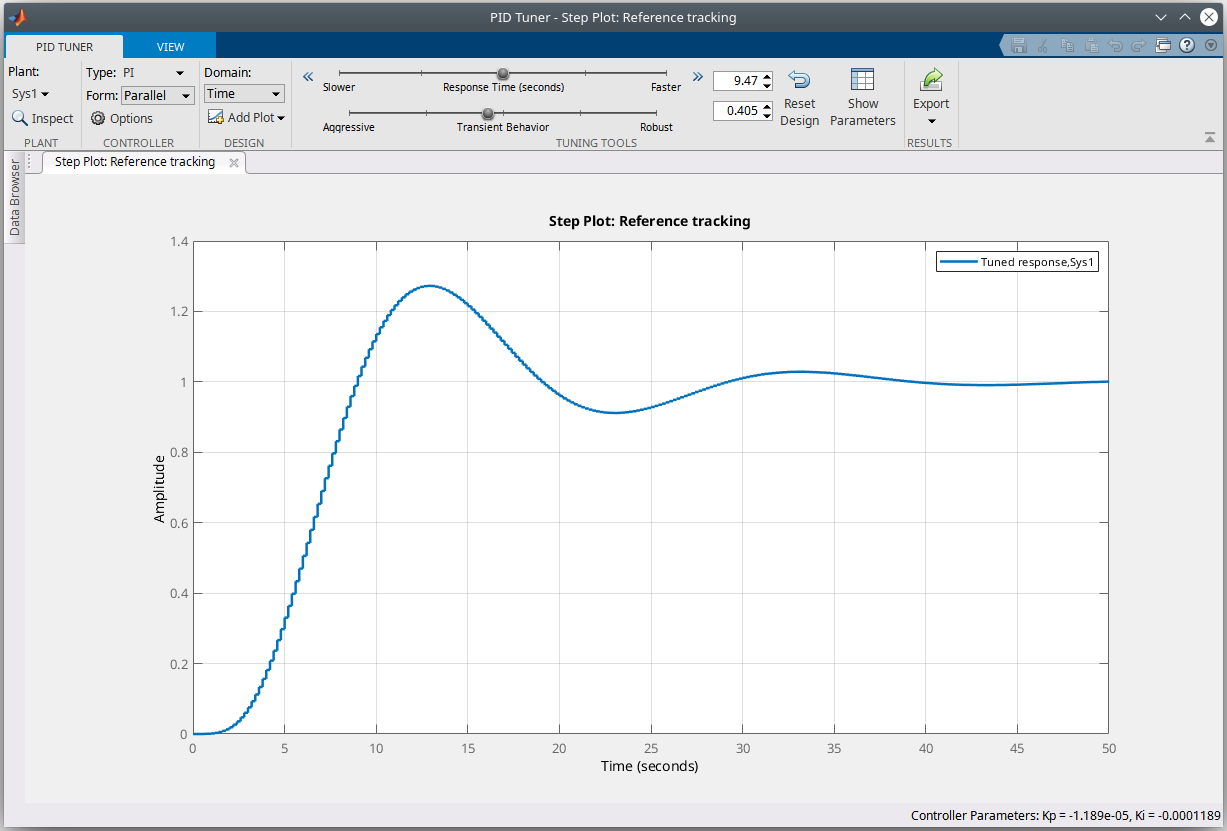
\includegraphics[width=\textwidth]{chap/Appendix/ControllerDesign/pidTuner}
	\caption[Matlab PID Tuner]{Screenshot of the Matlab PID Tuner from the Control Systems Toolbox}
	\label{fig:Appendix-pidTuner}
\end{figure}

\begin{figure}[H]
	\centering
	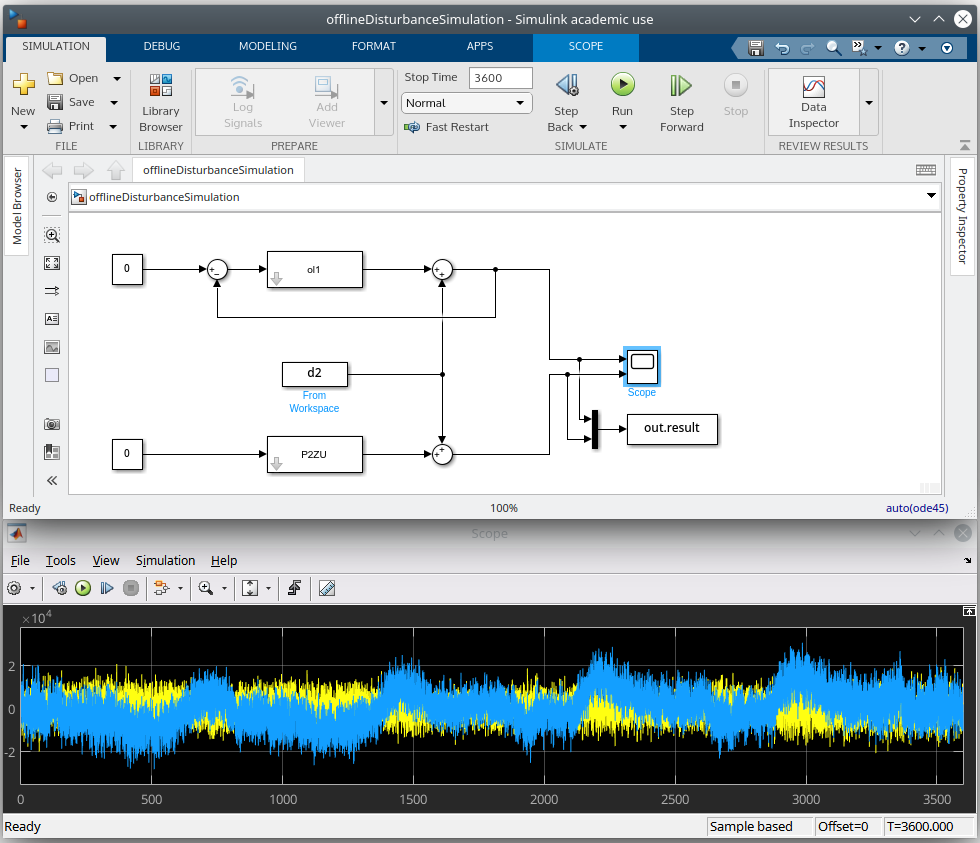
\includegraphics[width=\textwidth]{chap/Appendix/ControllerDesign/simulink}
	\caption[Simulink Model for Offline Evaluation]{Simulink model to evaluate the designed controller together with the measurement filter (\texttt{ol1}) compared to the uncontrolled system (in \texttt{P2ZU}) using measured disturbance data (in the vector \texttt{d2}); below a view of the scope data}
	\label{fig:Appendix-simuliunk}
\end{figure}

\begin{figure}[H]
	\centering
	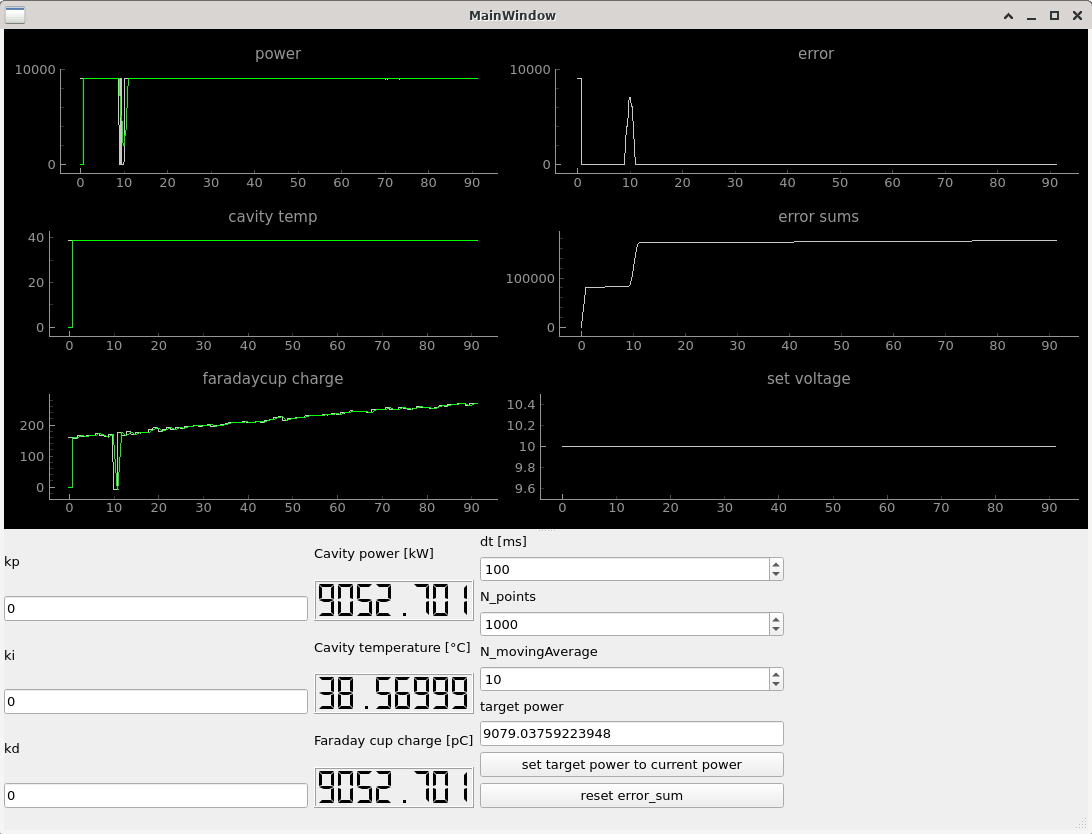
\includegraphics[width=\textwidth]{chap/Appendix/ControllerDesign/qt}
	\caption[Control System GUI]{Screenshot of the control system's GUI application}
	\label{fig:Appendix-qt}
\end{figure}

\FloatBarrier
\begin{lstlisting}[style=java,caption = Java class of the PCB421A25 charge amplifier demonstrating the command structure and checksum calculation for integration of the amplifier into \gls{css}, label = lst:Appendix-javaPcb]
class PCB421A25 {
	final static char STX = '\u0002';	
	static enum FixedRange {
		RANGE_1000000("01"), 
		RANGE_500000("02"),
		RANGE_200000("03"),
		RANGE_100000("04"),
		RANGE_50000("05"),
		RANGE_20000("06"),
		RANGE_10000("07"),
		RANGE_5000("08"),
		RANGE_2000("09"),
		RANGE_1000("10"),
		RANGE_500("11"),
		RANGE_200("12"),
		RANGE_100("13");
		public final String command;
		private FixedRange(String command) {
			this.command = command;
		}
	}
	
	public PCB421A25() {};
	
	public void setFixedRange(FixedRange fixedRange) {
		String command=STX+"c"+"0"+fixedRange.command;
		command += calculateChecksum(command);
		sendCommand(command);
	}
	
	public boolean setVariableRange(int variableRange) {
		if(!(variableRange>100 && variableRange<1000000)) return false;
		String command=STX+"d"+"0"+String.format("%06d", variableRange);
		command += calculateChecksum(command);
		sendCommand(command);
		return true;
	}
	
	private char calculateChecksum(String command) {
		int checksum=0;
		for(int i=0;i<command.length();i++)
			checksum+=(int)command.charAt(i);
		String checksum_hexstr=Integer.toHexString(checksum).toUpperCase();
		return checksum_hexstr.charAt(checksum_hexstr.length()-1);
	}
	
	private void sendCommand(String command){
		System.out.println("Command to send: "+command+" (length: "+command.length()+")");
		//[...]
	}
	
  public static void main(String[] args) {
		PCB421A25 chargeSensitiveAmplifier = new PCB421A25();
		
		//Test fixed ranges
		System.out.print("Fixed range 1000000;\t");
		chargeSensitiveAmplifier.setFixedRange(FixedRange.RANGE_1000000);
        System.out.print("Fixed range 100;\t");
        chargeSensitiveAmplifier.setFixedRange(FixedRange.RANGE_100);
        
        //Test variable ranges
		System.out.print("Variable range 123456;\t");
		chargeSensitiveAmplifier.setVariableRange(23500);
		System.out.print("Variable range 999;\t");
		chargeSensitiveAmplifier.setVariableRange(999);
    }
}
\end{lstlisting}